% Slides do Projeto Final - IF69D (PDI)
% Segmentacao de vasos em imagens de Doppler colorido
% Compilar: pdflatex apresentacao.tex (2x)
\documentclass[aspectratio=169,11pt]{beamer}

\usetheme{Madrid}
\usecolortheme{default}
\beamertemplatenavigationsymbolsempty

\usepackage[T1]{fontenc}
\usepackage[utf8]{inputenc}
\usepackage[brazil]{babel}
\usepackage{graphicx}
\usepackage{booktabs}
\usepackage{amsmath}

% caminho das figuras
\graphicspath{{imgs/}{imgs/phantom/}{imgs/ground_truth/}{imgs/compare_methods/}}

% --- metadados da capa ---
\title[Segmentação em Doppler colorido]{Segmentação de vasos em imagens de Doppler colorido}
\subtitle{Distância Euclidiana vs.\ K-means}
\author[Tronconi; Bubniak]{Etore Maloso Tronconi \and Henrique Gomes Pinto Bubniak}
\institute[UTFPR]{IF69D / OPEET014 -- Processamento Digital de Imagens\\Prof.\ Gustavo B.\ Borba -- UTFPR}
\date{junho de 2026}

\begin{document}

\begin{frame}[plain]
  \titlepage
\end{frame}

\begin{frame}{Roteiro}
  \tableofcontents
\end{frame}

% =====================================================================
\section{Objetivo}
\begin{frame}{Objetivo}
  \begin{block}{Meta do trabalho}
    Segmentar o vaso sanguíneo (fluxo se afastando da sonda, em \textbf{azul})
    \textbf{a partir da imagem de Doppler colorido} -- como se só existisse a
    figura na tela, sem acesso ao campo de velocidade bruto -- e avaliar
    quantitativamente a segmentação contra um \emph{ground truth}.
  \end{block}
  \begin{itemize}
    \item Comparar, de forma padronizada, dois métodos de segmentação por cor:
      \begin{itemize}
        \item \textbf{Distância Euclidiana} a uma cor de referência + Otsu;
        \item \textbf{K-means} no espaço de cor Lab.
      \end{itemize}
    \item Métricas objetivas: Dice, IoU, precisão e recall.
  \end{itemize}
\end{frame}

% =====================================================================
\section{Fundamentação Teórica}

\begin{frame}{Contexto e dados}
  \begin{columns}[c]
    \column{0.55\textwidth}
      \begin{itemize}
        \item Simulações de ultrassom Doppler (toolbox \textbf{MUST}) sobre
          \emph{phantoms} de vasos 128$\times$128.
        \item Cada \texttt{vd\_signals\_XX.mat} guarda o mapa de velocidade
          (m/s, \texttt{NaN} fora do feixe).
        \item O campo cobre o dobro da largura do phantom $\Rightarrow$
          recorta-se o \textbf{FOV central} antes de comparar.
        \item 15 simulações; \emph{ground truth} gerado dos phantoms
          (azul $\rightarrow$ branco).
      \end{itemize}
    \column{0.45\textwidth}
      \centering
      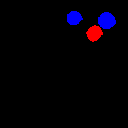
\includegraphics[width=0.6\textwidth]{vessels_03.png}\\
      \footnotesize Phantom (vasos azul/vermelho sobre fundo).
  \end{columns}
\end{frame}

\begin{frame}{Da velocidade à imagem colorida}
  \begin{columns}[c]
    \column{0.6\textwidth}
      \begin{itemize}
        \item O mapa de velocidade é renderizado com o \emph{colormap}
          \texttt{dopplermap} (MUST), como num \emph{scanner} clínico
          (\texttt{ind2rgb} + \texttt{caxis} simétrico).
        \item Codificação de cor:
          \begin{itemize}
            \item \textbf{Azul/ciano} -- fluxo se afastando da sonda (velocidade negativa, alvo);
            \item \textbf{Vermelho/amarelo} -- fluxo se aproximando (velocidade positiva);
            \item \textbf{Preto} -- velocidade $\approx 0$ (fundo, maioria da imagem).
          \end{itemize}
        \item O fundo escuro facilita isolar o vaso pela cor.
      \end{itemize}
    \column{0.4\textwidth}
      \centering
      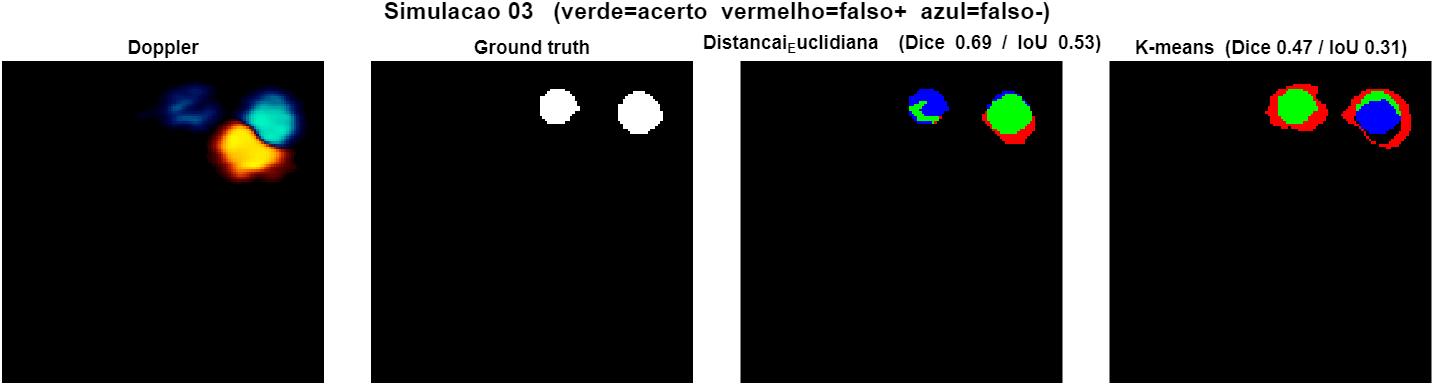
\includegraphics[width=0.95\textwidth]{cmp_03.png}\\
      \footnotesize Doppler renderizado e segmentações.
  \end{columns}
\end{frame}

\begin{frame}{Método 1 -- Distância Euclidiana + Otsu}
  \begin{itemize}
    \item Cor de referência do alvo: \textbf{média interquartílica} dos canais de
      uma pequena amostra (\texttt{sample.png}), robusta a \emph{outliers}.
    \item Distância de cada pixel $\mathbf{x}$ à referência $\boldsymbol{\mu}$:
      \begin{equation*}
        D(\mathbf{x}) = \sqrt{\sum_{c \in \{R,G,B\}} \big(I_c(\mathbf{x}) - \mu_c\big)^2}
      \end{equation*}
    \item Limiarização automática por \textbf{Otsu} sobre o mapa de distância:
      pixels com $D(\mathbf{x}) < t$ são marcados como vaso.
  \end{itemize}
\end{frame}

\begin{frame}{Método 2 -- K-means (espaço Lab)}
  \begin{itemize}
    \item Agrupamento das cores em \textbf{K = 3} \emph{clusters} com
      \texttt{imsegkmeans}, no espaço \textbf{Lab} (separa cor de luminância
      melhor que RGB).
    \item Cada cluster captura naturalmente uma região: azul, vermelho e fundo.
    \item Seleciona-se o cluster com o canal \textbf{$b^\ast$ (Lab) mais negativo}
      -- ou seja, o mais azul (critério intrínseco, sem depender da amostra).
    \item Tende a recuperar todo o vaso (\emph{recall} alto), mas pode incluir
      transições ao redor (precisão menor).
  \end{itemize}
\end{frame}

\begin{frame}{Métricas de avaliação}
  Comparação pixel a pixel da máscara obtida com o \emph{ground truth}
  ($\mathrm{TP}$, $\mathrm{FP}$, $\mathrm{FN}$):
  \begin{columns}[t]
    \column{0.5\textwidth}
      \begin{align*}
        \mathrm{Dice} &= \frac{2\,\mathrm{TP}}{2\,\mathrm{TP}+\mathrm{FP}+\mathrm{FN}} \\[4pt]
        \mathrm{IoU}  &= \frac{\mathrm{TP}}{\mathrm{TP}+\mathrm{FP}+\mathrm{FN}}
      \end{align*}
    \column{0.5\textwidth}
      \begin{align*}
        \text{Precisão} &= \frac{\mathrm{TP}}{\mathrm{TP}+\mathrm{FP}} \\[4pt]
        \text{Recall} &= \frac{\mathrm{TP}}{\mathrm{TP}+\mathrm{FN}}
      \end{align*}
  \end{columns}
  \vspace{0.4em}
  \begin{itemize}
    \item Dice e IoU calculados com as funções nativas \texttt{dice} e \texttt{jaccard}.
    \item \emph{Ground truth}: pixels azuis do phantom $\rightarrow$ branco; resto $\rightarrow$ preto.
  \end{itemize}
\end{frame}

% =====================================================================
\section{Implementação}

\begin{frame}{Pipeline padronizado}
  \centering
  \footnotesize
  \fbox{\parbox{2.2cm}{\centering Mapa de\\velocidade (VD)}}\;$\Rightarrow$\;
  \fbox{\parbox{2.4cm}{\centering Render \texttt{dopplermap}\\+ recorte FOV}}\;$\Rightarrow$\;
  \fbox{\parbox{2.2cm}{\centering Suavização\\Gaussiana}}\;$\Rightarrow$\;
  \fbox{\parbox{2.3cm}{\centering Segmentação\\(Dist.\ / K-means)}}\;$\Rightarrow$\;
  \fbox{\parbox{2.2cm}{\centering Pós-proc.\\(fechamento)}}\;$\Rightarrow$\;
  \fbox{\parbox{2.1cm}{\centering Métricas\\vs.\ \emph{GT}}}

  \vspace{1.2em}
  \normalsize
  \begin{block}{Padronização da comparação}
    Os dois métodos partem da \textbf{mesma imagem}, com o \textbf{mesmo pré}
    (suavização Gaussiana) e \textbf{pós-processamento} (fechamento morfológico
    + preenchimento de buracos); só muda o passo de segmentação. Assim a
    comparação é justa.
  \end{block}
\end{frame}

\begin{frame}{Arquivos e funções (MATLAB)}
  \begin{itemize}
    \item \texttt{doppler\_to\_rgb.m} -- VD $\rightarrow$ imagem \texttt{dopplermap}
      128$\times$128 (renderização comum).
    \item \texttt{segment\_doppler.m} -- roda os métodos:
      \begin{itemize}
        \item \texttt{euclidia\_limiar} -- distância Euclidiana + Otsu;
        \item \texttt{seg\_kmeans} -- \texttt{imsegkmeans} no Lab.
      \end{itemize}
    \item \texttt{make\_ground\_truth.m} -- gera as máscaras de referência.
    \item \texttt{eval\_methods.m} -- avaliação dos 15 casos, tabela, veredito e painéis.
  \end{itemize}
  \vspace{0.3em}
  \textbf{Funções nativas usadas:} \texttt{rgb2lab}, \texttt{imsegkmeans},
  \texttt{graythresh}, \texttt{imgaussfilt}, \texttt{dice}, \texttt{jaccard}.
  \vspace{0.5em}

  \footnotesize \textbf{Como rodar:} \texttt{make\_ground\_truth} $\rightarrow$ \texttt{eval\_methods}.
\end{frame}

% =====================================================================
\section{Resultados e conclusões}

\begin{frame}{Resultados quantitativos (15 simulações)}
  \begin{columns}[c]
    \column{0.46\textwidth}
      \centering
      \begin{table}
        \footnotesize
        \begin{tabular}{lcc}
          \toprule
          \textbf{Métrica} & \textbf{Dist.\ Euclid.} & \textbf{K-means} \\
          \midrule
          Dice      & \textbf{0,698} & 0,588 \\
          IoU       & \textbf{0,544} & 0,426 \\
          Precisão  & \textbf{0,598} & 0,436 \\
          Recall    & 0,873 & \textbf{0,964} \\
          \bottomrule
        \end{tabular}
        \caption{Médias por método.}
      \end{table}
      \textbf{Distância Euclidiana vence em 14 de 15 imagens} (Dice por imagem).
    \column{0.54\textwidth}
      \centering
      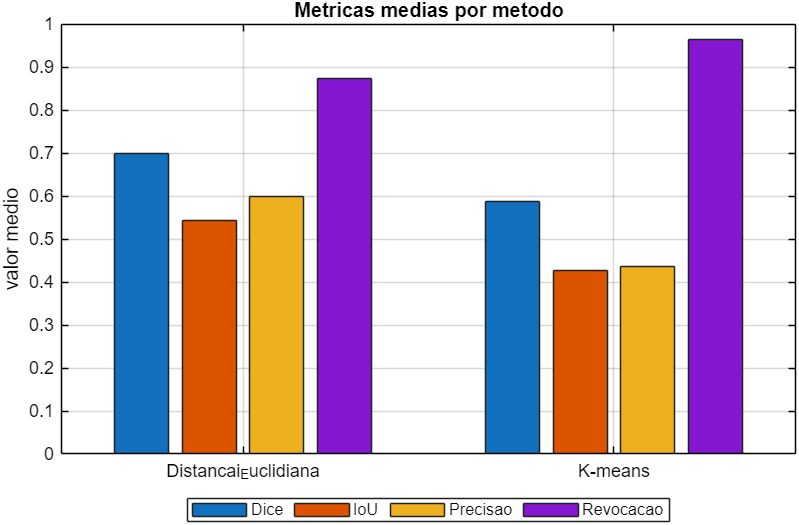
\includegraphics[width=0.95\textwidth]{summary.png}\\
      \footnotesize Médias por método.
  \end{columns}
\end{frame}

\begin{frame}{Resultados qualitativos}
  \centering
  \footnotesize verde = acerto \quad vermelho = falso positivo \quad azul = falso negativo
  \begin{columns}[c]
    \column{0.5\textwidth}
      \centering
      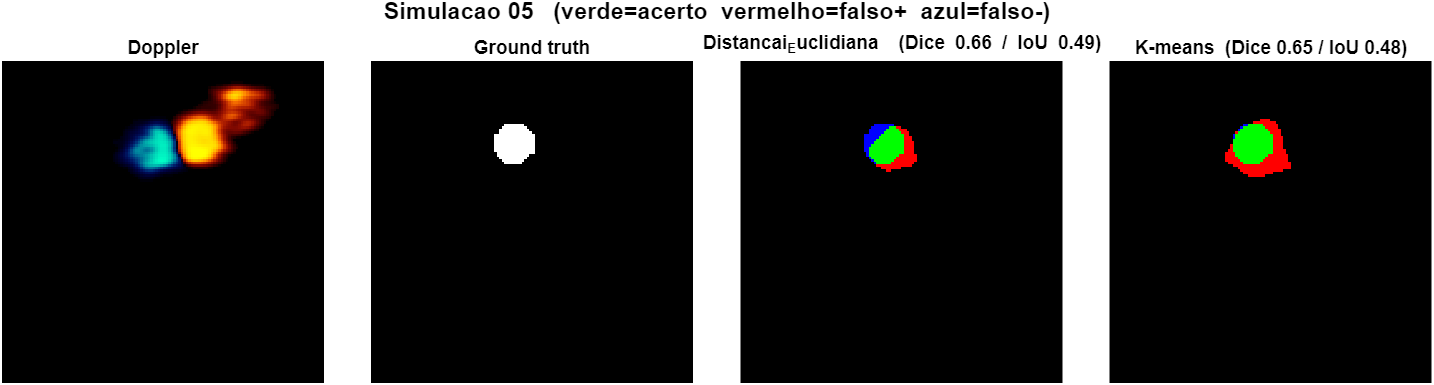
\includegraphics[width=\textwidth]{cmp_05.png}\\
      \footnotesize Exemplo de comparação (1).
    \column{0.5\textwidth}
      \centering
      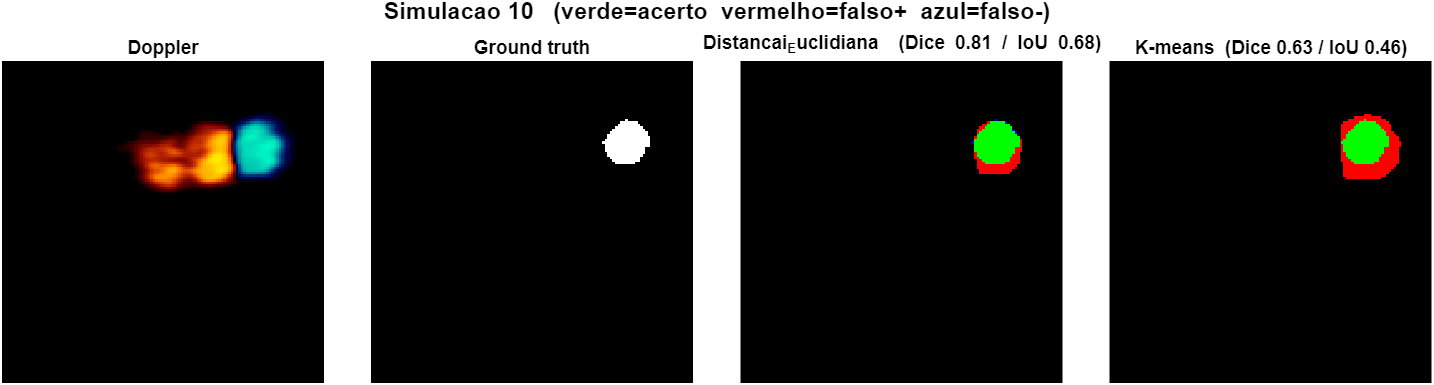
\includegraphics[width=\textwidth]{cmp_10.png}\\
      \footnotesize Exemplo de comparação (2).
  \end{columns}
  \vspace{0.3em}
  \begin{center}
    {\footnotesize Fundo preto do \texttt{dopplermap} facilita isolar o vaso pela cor.}
  \end{center}
\end{frame}

\begin{frame}{Conclusões e melhorias futuras}
  \begin{block}{Conclusões}
    \begin{itemize}
      \item A \textbf{Distância Euclidiana} foi o melhor método (Dice 0,70 vs.\ 0,59;
        vence em 14/15), com bom equilíbrio entre precisão (0,60) e recall (0,87).
      \item O \textbf{K-means} tem \emph{recall} altíssimo (0,96), mas precisão baixa
        (0,44): \textbf{sobre-segmenta} -- o cluster azul engloba transições e
        excesso ao redor do vaso.
      \item O fundo preto do \texttt{dopplermap} facilitou a segmentação por cor.
    \end{itemize}
  \end{block}
  \begin{block}{Melhorias propostas}
    \begin{itemize}
      \item Reduzir a sobre-segmentação do K-means (refinar a seleção do cluster
        ou aumentar $K$);
      \item Pós-processamento adicional: abertura morfológica e seleção do maior
        componente conexo como vaso;
      \item Classificação pela \textbf{referência mais próxima} (azul vs.\ vermelho).
    \end{itemize}
  \end{block}
  \vfill
  {\tiny Fonte da fundamentação teórica: slides das Aulas 05/09/10 da disciplina IF69D -- Prof.\ Gustavo B.\ Borba.}
\end{frame}

\begin{frame}[plain]
  \centering
  \vfill
  {\Large Obrigado!}\\[1em]
  {\normalsize Etore Maloso Tronconi \quad$\cdot$\quad Henrique Gomes Pinto Bubniak}
  \vfill
\end{frame}

\end{document}
